\documentclass[conference]{IEEEtran}
\usepackage[T1]{fontenc}
\usepackage{cite}
\usepackage{amsmath,amssymb}
\usepackage{graphicx}
\usepackage{booktabs,array}
\usepackage{url,balance}
\usepackage[hidelinks]{hyperref}
\hypersetup{pdftitle={Liquidity-Aware Price-Deviation Detection with Explainable Evidence for Colombo Stock Exchange Equities},pdfauthor={S. A. H. Samarathunga; K. C. S. Fernando; Harithra K; T. G. R. N. S. Wijesooriya; Kapila Dissanayaka; Mahima Weerasinghe}}
\graphicspath{{figures/}}
\hyphenation{li-quid-ity fore-cast fore-cast-ing}

\title{Liquidity-Aware Price-Deviation Detection with Explainable Evidence for Colombo Stock Exchange Equities}
\author{
\IEEEauthorblockN{S. A. H. Samarathunga}
\IEEEauthorblockA{\textit{Faculty of Computing}\\
Sri Lanka Institute of Information\\Technology\\Malabe, Sri Lanka\\
it21296482@my.sliit.lk}
\and
\IEEEauthorblockN{K. C. S. Fernando}
\IEEEauthorblockA{\textit{Faculty of Computing}\\
Sri Lanka Institute of Information\\Technology\\Malabe, Sri Lanka\\
it21471162@my.sliit.lk}
\and
\IEEEauthorblockN{Harithra K}
\IEEEauthorblockA{\textit{Faculty of Computing}\\
Sri Lanka Institute of Information\\Technology\\Malabe, Sri Lanka\\
it22065308@my.sliit.lk}
\and
\IEEEauthorblockN{T. G. R. N. S. Wijesooriya}
\IEEEauthorblockA{\textit{Faculty of Computing}\\
Sri Lanka Institute of Information\\Technology\\Malabe, Sri Lanka\\
it22547088@my.sliit.lk}
\and
\IEEEauthorblockN{Kapila Dissanayaka}
\IEEEauthorblockA{\textit{Faculty of Computing}\\
Sri Lanka Institute of Information\\Technology\\Malabe, Sri Lanka}
\and
\IEEEauthorblockN{Mahima Weerasinghe}
\IEEEauthorblockA{\textit{Faculty of Computing}\\
Sri Lanka Institute of Information\\Technology\\Malabe, Sri Lanka}
}

\begin{document}
\maketitle
\begin{abstract}
An observed stock-price change does not reveal whether the movement is unusual or how reliable its explanation is. This paper presents a liquidity-aware evidence workflow for the Colombo Stock Exchange, combining recurrent expected-price estimation, a volume-adjusted residual, a calibrated prediction-band rule and surrogate additive feature explanations. Rolling top-factor overlap describes explanation stability. Evaluation uses preserved John Keells Holdings and Browns Investments histories and 57 matched dates per stock for a separate three-month forecast comparison. Ensemble mean absolute percentage errors were 7.07\% and 15.83\%, against unchanged-price baseline errors of 2.74\% and 11.76\%. For John Keells Holdings, the deviation detector recovered eight of nine proxy anomalies but raised 30 false alarms; its precision--recall harmonic mean was 0.3404, below the statistical baseline's 0.7500. Mean explanation-factor overlap was 0.896552 and 1.0 for the respective stocks, alongside strong volume-feature dominance. These findings support an auditable research workflow rather than predictive superiority. Retrospective proxy labels, two-stock coverage and unverified forecast-registration timing limit generalisation. The contribution separates observed unusualness, historical-pattern gaps and forecast uncertainty within an integrated investor-facing system.
\end{abstract}
\begin{IEEEkeywords}
Colombo Stock Exchange, anomaly detection, liquidity-aware deviation, time-series forecasting, explainable artificial intelligence
\end{IEEEkeywords}

\section{Introduction}
A falling share price may reflect ordinary variation, an exceptional departure from recent behaviour or a sustained shift that is no longer unusual day by day. Participation matters: an identical price gap can occur on thin trading or broad activity. Displaying a forecast alone leaves these distinctions unresolved.

This work addresses the market-modelling contribution to the AI-Powered Stock Market Insight Generator for the Colombo Stock Exchange (CSE). Its research question is whether expected-price estimation, participation-aware deviations and traceable explanations can be combined into inspectable evidence. The objective is decision support, not automatic trading. A complex estimate must still be compared with an unchanged-price baseline.

The contribution is threefold: (i) a volume-adjusted residual joined with a separately calibrated band alert; (ii) surrogate feature attributions accompanied by a rolling top-three explanation-overlap statistic; and (iii) reproducible evaluation that exposes baseline failures, false alarms and uncertainty. Historical-pattern gaps remain separate from daily anomaly flags. Long short-term memory (LSTM), random forests and Shapley additive explanations (SHAP) are established methods, not new algorithms claimed here. Other project contributions supply report interpretation, news/sentiment and external-market risk; their independent performance is outside this paper's evaluation.

\section{Related Work}
LSTM supports sequence learning \cite{hochreiter}; Fischer and Krauss investigated its use for financial direction prediction \cite{fischer}. That task and market population differ from CSE price-level estimation. Benchmark comparisons and the distinction between one-step residuals and multi-step forecasts therefore remain necessary \cite{hyndmanbook}. Forecast-error measures also require careful interpretation \cite{hyndmankoehler}: $100-\mathrm{MAPE}$ is not a probability of correctness.

Anomaly detection depends on the definition of normality and the available labels \cite{chandola}. Isolation Forest isolates unusual observations through random partitions \cite{isolation}; we compare it and a statistical Z-score with the proposed residual rule. Amihud's measure relates absolute returns to monetary trading volume \cite{amihud}. Our score differs: it divides a model price residual by share volume. It is price-scale dependent, requires stock-specific calibration and is not a causal price-impact measure. Rare-event evaluation must expose precision and recall rather than rely on accuracy alone \cite{saito}.

SHAP provides additive feature attributions \cite{shap}, with Tree SHAP supporting tree ensembles \cite{treeshap}. Here, a random forest \cite{breiman} approximates the anomaly score. Explaining that surrogate does not directly explain LSTM internals. Consistent with the distinction between technical explanations and human understanding \cite{miller}, we do not infer investor comprehension or trust from attribution plots alone.

\section{Methodology}
\subsection{Data Flow and Expected Price}
Fig.~\ref{fig:architecture} outlines the workflow. Dated OHLCV records are checked for duplicates, non-positive prices, inconsistent ranges and negative volume; unavailable observations are not replaced with invented prices. Features include returns, moving averages, volatility, momentum, range, RSI, ATR and relative volume. Preserved records identify a TradingView CSELK fallback, not an independently verified exchange-only history.

\begin{figure*}[!t]
\centering
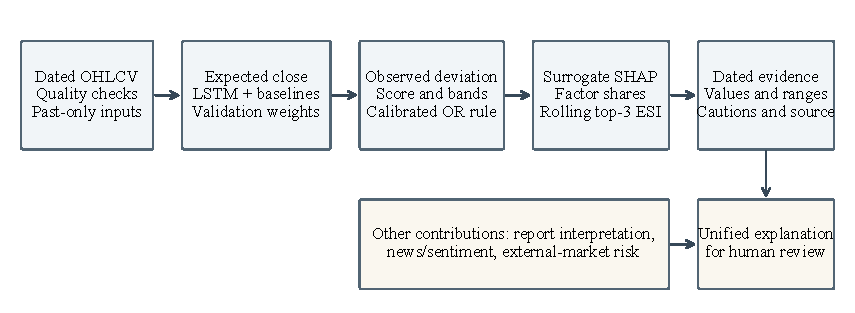
\includegraphics[width=\textwidth]{architecture.pdf}
\caption{Market-evidence workflow and integration boundary. Other contributions provide report, news/sentiment and external-risk evidence; synthesis does not alter the market calculations.}
\label{fig:architecture}
\end{figure*}

Let $A_t$ denote the observed close, $V_t$ share volume and $\mathbf{x}_t$ engineered features. The expected close is
\begin{equation}
P_t=f_{\theta}(\mathbf{x}_{t-20},\ldots,\mathbf{x}_{t-1}).
\label{eq:predict}
\end{equation}
The scaler is fitted on training rows only. Chronological validation supports calibration; later test rows assess the selected model. This is rolling one-step prediction, not a single-origin multi-month forecast.

The retained LSTM uses two 32-unit layers, dropout 0.15, a maximum of 12 epochs, batch size 32 and early stopping after four non-improving validation epochs. Adam \cite{adam} uses learning rate $10^{-3}$ and weight decay $10^{-5}$ with mean squared error, restoring the best validation state. These are archived settings, not later application defaults.

The separate preserved multi-step scenario combines LSTM, unchanged-price and moving-average-drift paths:
\begin{equation}
w_i=\frac{1/\max(e_i,\epsilon_w)}{\sum_j1/\max(e_j,\epsilon_w)},\quad
\widehat A_{t+h}=\sum_iw_i\widehat A_{t+h}^{(i)},
\label{eq:ensemble}
\end{equation}
where $e_i$ is validation MAE and $\epsilon_w=10^{-6}$. Future forecasts $\widehat A_{t+h}$ must not replace $P_t$ when assessing an already observed date.

\subsection{Deviation and Liquidity-Aware Score}
Direction and magnitude are preserved as
\begin{equation}
D_t=A_t-P_t,\quad d_t=|A_t-P_t|,\quad
\delta_t=100\frac{A_t-P_t}{P_t}.
\label{eq:deviation}
\end{equation}
For $P_t>0$, $\delta_t$ is a percentage relative to expectation; $D_t$ and $d_t$ are in LKR. The participation-aware score is
\begin{equation}
v_t=V_t/10^6,\qquad S_t=\frac{d_t}{v_t+\epsilon},\qquad\epsilon=10^{-6}.
\label{eq:score}
\end{equation}
Less volume increases the score for the same price gap. It is neither a percentage nor a risk probability. Zero-volume observations are unreliable and cannot independently trigger its liquidity alert.

Illustratively, $P_t=24.00$, $A_t=19.80$ and $V_t=2$ million give $D_t=-4.20$ LKR, $\delta_t=-17.50\%$ and $S_t\approx2.10$. These are example inputs, not a current quote or fair-value estimate. Fig.~\ref{fig:sensitivity} shows the volume dependence.

\begin{figure}[!t]
\centering
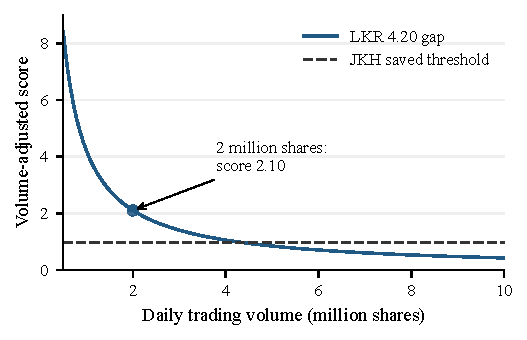
\includegraphics[width=\columnwidth]{score_sensitivity.pdf}
\caption{Illustrative LKR 4.20 gap: the score crosses the saved JKH threshold near 4.37 million shares. A separate band alert can still occur.}
\label{fig:sensitivity}
\end{figure}

Relative volume is $u_t=V_t/\operatorname{median}_{20}(V)$. Low volume means $u_t<0.50$; thin trading means $u_t<0.25$ or $V_t=0$. The complementary diagnostic $C_t=d_t\ln(1+v_t)$ increases with participation but is excluded from the final rule. These are observed-day checks, not quantities known before that session ends.

\subsection{Bands, Thresholds and Proxy Labels}
Validation residuals determine downside/upside widths $b_-,b_+$. Each is at least the maximum of the 95th percentile of absolute residuals, their population standard deviation and $10^{-6}$, and its corresponding one-sided 95th-percentile gap. Define
\begin{equation}
B_t=\max\left(\frac{\max(P_t-A_t,0)}{b_-},\frac{\max(A_t-P_t,0)}{b_+}\right),
\label{eq:band}
\end{equation}
\begin{equation}
a_t=\mathbb{1}\left[(S_t\ge T_S\land V_t>0)\lor(B_t\ge T_B)\right].
\label{eq:flag}
\end{equation}
Liquidity candidates span training/validation score quantiles 0.60--0.995; band candidates have minimum severity 1.05. Pairs maximise validation
\begin{equation}
F_{0.5}=\frac{1.25\,\mathrm{Pr}\,\mathrm{Re}}{0.25\,\mathrm{Pr}+\mathrm{Re}},
\label{eq:fbeta}
\end{equation}
where $\mathrm{Pr}=TP/(TP+FP)$ and $\mathrm{Re}=TP/(TP+FN)$. Ties favour precision, controlled flag rates, rate consistency, accuracy and recall. Thresholds are stock/run-specific; precision emphasis is a design preference, not measured investor utility.

Retained proxy labels mark predefined stress windows or extreme absolute returns (97.5th percentile) accompanied by high 20-day volatility or a volume-to-mean spike (90th percentiles). Windows are 22 April--10 May 2019, 9 March--15 May 2020 and 1 March--31 July 2022. An audit reproduced all archived test labels with full-history quantiles. Thus, later observations affect the target definition: these are retrospective proxy-label comparisons, not leakage-free prospective event-detection results. Later past-only rolling labels are not substituted into these scores.

\subsection{Pattern Context and Explainability}
To distinguish daily unusualness from a persistent pattern gap, define
\begin{align}
R_t&=0.35\,\mathrm{SMA}_{20,t}+0.25\,\mathrm{SMA}_{50,t}\nonumber\\
&\quad+0.25\,\mathrm{EMA}_{12,t}+0.15P_t,\\
g_t&=\max(R_t-A_t,0)/R_t.
\label{eq:pattern}
\end{align}
Missing averages fall back to $P_t$; a positive-gap cutoff uses training/validation fractions. This observed-day reference is not fundamental value or a recovery guarantee; its flag is not OR-ed into (\ref{eq:flag}). Separate pressure is $\Pi_t=\sum_j|(x_{j,t}-\mu_j)/\sigma_j|$ over returns, volatility, volume ratio and $S_t$, with training/validation reference statistics. It does not identify the causal effect of news or war.

A 300-tree random-forest surrogate, minimum leaf size five and seed 42, estimates $S_t$ from nine features: volume-to-20-day-mean ratio, 20-day volatility, 10-day momentum, moving-average gap, one-day return, range fraction, open-to-close change, RSI(14) and ATR(14). Training/validation rows fit the surrogate. Tree SHAP yields
\begin{equation}
f_s(\mathbf{x}_t)=\phi_0+\sum_j\phi_{j,t},\qquad
p_{j,t}=\frac{|\phi_{j,t}|}{\sum_k|\phi_{k,t}|}.
\label{eq:shap}
\end{equation}
Signed contributions describe direction relative to the surrogate baseline; $p_{j,t}$ retains magnitude only. They explain the score surrogate, not LSTM gates or causal price drivers. A feature-importance fallback is explicitly labelled if SHAP is unavailable.

For 60-observation windows advancing by 20, let $K_w$ contain the three factors ranked highest by mean absolute SHAP value. Explanation stability is
\begin{equation}
\mathrm{ESI}_w=|K_w\cap K_{w-1}|/3.
\label{eq:esi}
\end{equation}
Two shared names give $2/3$; values $\ge0.80$ are high, $[0.50,0.80)$ moderate and lower values low. ESI measures membership overlap, not sign, magnitude, fidelity or comprehension; fewer than two windows cannot establish stability.

\section{Evaluation and Results}
\subsection{Protocol and Measures}
Table~\ref{tab:data} summarises the histories. JKH is John Keells Holdings PLC (JKH.N0000); BIL is Browns Investments PLC (BIL.N0000). Feature warm-up and sequence construction precede the approximately 70/10/20\% chronological split. The JKH test spans 16 August 2023--7 May 2026; BIL spans 20 September 2023--7 May 2026.

\begin{table}[!t]
\caption{Preserved Histories and Evaluation Samples}
\label{tab:data}
\centering\footnotesize
\begin{tabular}{@{}lrr@{}}\toprule
Attribute & JKH & BIL\\\midrule
First raw date & 22 Feb. 2012 & 23 Feb. 2012\\
Last raw date & 7 May 2026 & 7 May 2026\\
Raw OHLCV rows & 3,308 & 3,238\\
One-step test rows & 647 & 629\\
Test proxy positives & 9 & 2\\
Matched scenario dates & 57 & 57\\\bottomrule
\end{tabular}
\end{table}

The separate scenario covers 60 business-day targets, 8 May--30 July 2026. Actuals match 57 dates per stock; missing 28 May, 29 June and 29 July observations are excluded, not interpolated or assumed exchange closures. The record dates forecast preservation to 10 May, after the first target. This is an evaluation of preserved forecasts against later-obtained observations, not independently preregistered prospective validation.

For errors $e_t=\widehat A_t-A_t$ on $n$ matched dates,
\begin{align}
\mathrm{MAE}&=n^{-1}\sum_t|e_t|,\quad
\mathrm{RMSE}=\sqrt{n^{-1}\sum_te_t^2},\nonumber\\
\mathrm{MAPE}&=100n^{-1}\sum_t|e_t|/|A_t|.
\label{eq:errors}
\end{align}
Interval coverage is the percentage of actuals inside the bounds; sharpness is mean width in LKR. Scenario intervals differ from one-step anomaly bands. Anomaly comparisons report accuracy $(TP+TN)/N$, precision, recall, $F1=2TP/(2TP+FP+FN)$ and confusion counts against archived proxies. An always-normal reference exposes imbalance. Input fingerprints and scripts reproduce arithmetic from saved outputs, not fitted neural weights, which were not preserved.

\subsection{Forecast Accuracy and Interval Quality}
Table~\ref{tab:forecast} and Fig.~\ref{fig:forecast} show that no change outperformed the ensemble and LSTM for both stocks. JKH ensemble MAE was 1.4157 LKR versus 0.5474 for persistence; BIL values were 0.8822 versus 0.6561. MAPE was 7.07\% versus 2.74\% for JKH and 15.83\% versus 11.76\% for BIL. Validation weighting did not prevent upward bias.

\begin{table}[!t]
\caption{Scenario Errors on 57 Matched Dates per Stock}
\label{tab:forecast}
\centering\footnotesize\setlength{\tabcolsep}{3pt}
\begin{tabular}{@{}llrrr@{}}\toprule
Stock & Path & MAE (LKR) & RMSE (LKR) & MAPE (\%)\\\midrule
JKH & Ensemble & 1.4157 & 1.5940 & 7.07\\
& LSTM & 1.1090 & 1.2599 & 5.54\\
& No change & \textbf{0.5474} & \textbf{0.6170} & \textbf{2.74}\\
& MA drift & 2.5342 & 2.8753 & 12.64\\\midrule
BIL & Ensemble & 0.8822 & 0.9884 & 15.83\\
& LSTM & 0.8565 & 0.9631 & 15.38\\
& No change & \textbf{0.6561} & \textbf{0.7276} & \textbf{11.76}\\
& MA drift & 1.1420 & 1.2864 & 20.50\\\bottomrule
\end{tabular}
\end{table}

\begin{figure*}[!t]
\centering
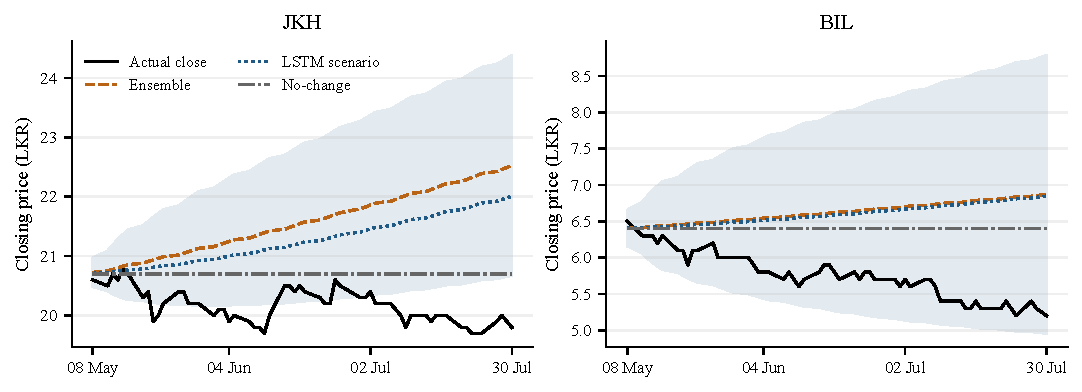
\includegraphics[width=\textwidth]{forecast_paths.pdf}
\caption{Preserved paths and actual closes on 57 matched dates, 8 May--30 July 2026. Shading is the ensemble's nominal 80\% range. Lines join recorded dates; no missing actuals were filled.}
\label{fig:forecast}
\end{figure*}

At 30 July, ensemble estimates were 22.5275 LKR against 19.80 for JKH, and 6.8708 against 5.20 for BIL: overestimates of 13.78\% and 32.13\% relative to actual prices. Actual closes fell 3.88\% and 20.00\% between the first and last matched dates. This identifies forecast error, not the cause of the declines.

Fig.~\ref{fig:intervals} pairs coverage with width. JKH's nominal 80\% range covered only 22/57 outcomes (38.60\%); its 95\% range covered all dates but averaged 8.91 LKR wide. BIL's 80\% and 95\% ranges covered all outcomes, with mean widths 2.57 and 5.61 LKR. Full coverage of broad ranges does not establish useful precision. Baseline failures and uncertainty must therefore remain visible to the user.

\begin{figure*}[!t]
\centering
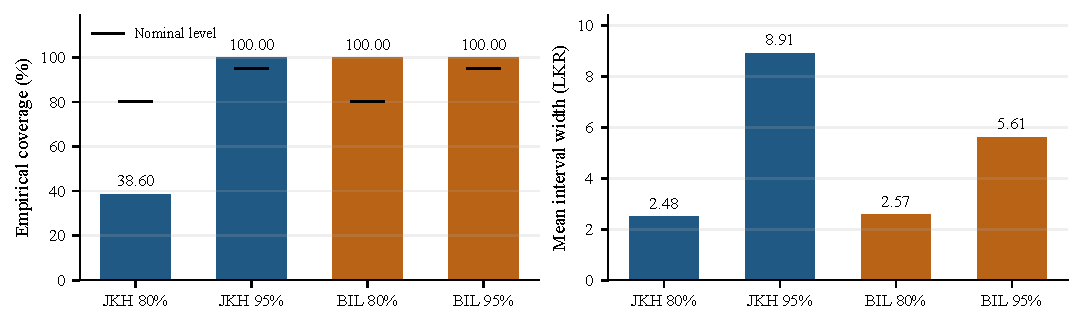
\includegraphics[width=\textwidth]{interval_quality.pdf}
\caption{Preserved-interval coverage and mean width. Black ticks show nominal coverage. Undercoverage and excessive width are distinct weaknesses; widths are not scale-normalised across stocks.}
\label{fig:intervals}
\end{figure*}

\subsection{Anomaly Detection and Calibration}
Table~\ref{tab:anomalies} exposes the operating trade-off. The deviation method detected eight of nine JKH positives (88.89\% recall) but raised 30 false alarms, giving 21.05\% precision and F1 0.3404. The Z-score detected six with one false alarm and F1 0.7500. Isolation Forest detected six with 17 false alarms and F1 0.3750. Greater recall did not produce the best F1.

\begin{table*}[!t]
\caption{Descriptive Test Comparisons Against Retrospective Proxy Labels}
\label{tab:anomalies}
\centering\footnotesize
\begin{tabular}{@{}llrrrrrrrr@{}}\toprule
Stock & Detector & Accuracy (\%) & Precision (\%) & Recall (\%) & F1 & TP & FP & FN & TN\\\midrule
JKH & Z-score & 99.38 & 85.71 & 66.67 & \textbf{0.7500} & 6 & 1 & 3 & 637\\
& Isolation Forest & 96.91 & 26.09 & 66.67 & 0.3750 & 6 & 17 & 3 & 621\\
& LSTM deviation & 95.21 & 21.05 & 88.89 & 0.3404 & 8 & 30 & 1 & 608\\
& Always normal & 98.61 & 0.00 & 0.00 & 0.0000 & 0 & 0 & 9 & 638\\\midrule
BIL & Z-score & 99.84 & 100.00 & 50.00 & \textbf{0.6667} & 1 & 0 & 1 & 627\\
& Isolation Forest & 99.84 & 100.00 & 50.00 & \textbf{0.6667} & 1 & 0 & 1 & 627\\
& LSTM deviation & 99.36 & 25.00 & 50.00 & 0.3333 & 1 & 3 & 1 & 624\\
& Always normal & 99.68 & 0.00 & 0.00 & 0.0000 & 0 & 0 & 2 & 627\\\bottomrule
\end{tabular}
\par\smallskip\parbox{\textwidth}{\footnotesize Archived labels are not independent event ground truth. Bold denotes greatest retained F1 per stock, not statistical superiority. Zero precision for always-normal predictions follows the implementation's zero-denominator convention.}
\end{table*}

For BIL, each nontrivial detector found one of only two positives. The deviation rule added three false alarms; Z-score and Isolation Forest added none. Changing one detection changes recall by 50 percentage points. Always-normal accuracy was 98.61\% for JKH and 99.68\% for BIL despite detecting no anomalies (Fig.~\ref{fig:confusion}). Accuracy alone is therefore insufficient.

\begin{figure}[!t]
\centering
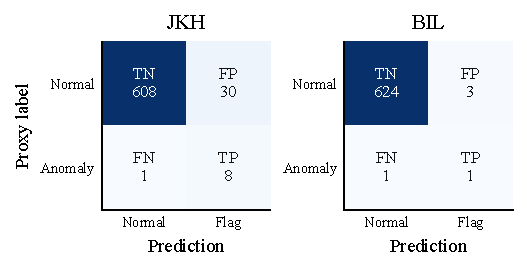
\includegraphics[width=\columnwidth]{confusion_matrices.pdf}
\caption{Saved deviation-method confusion counts. Rows are proxy labels, not verified market events.}
\label{fig:confusion}
\end{figure}

Table~\ref{tab:calibration} shows distinct stock-specific liquidity cutoffs. JKH's four liquidity and 34 band flags did not overlap; BIL's one and three did not overlap. These counts are diagnostics of the jointly tuned rule, not separately optimised ablations. Validation/test proxy prevalence also changed: 83/323 to 9/647 for JKH and 40/314 to 2/629 for BIL. Validation precision must not be advertised as future precision.

\begin{table}[!t]
\caption{Saved Calibration and Rule-Count Diagnostics}
\label{tab:calibration}
\centering\footnotesize
\begin{tabular}{@{}lrr@{}}\toprule
Quantity & JKH & BIL\\\midrule
Liquidity threshold $T_S$ & 0.961452 & 0.302219\\
Band threshold $T_B$ & 1.05 & 1.05\\
Validation precision & 0.7917 & 0.5714\\
Validation recall & 0.2289 & 0.2000\\
Validation $F_{0.5}$ & 0.5307 & 0.4167\\
Test liquidity / band flags & 4 / 34 & 1 / 3\\
Test overlap / final alerts & 0 / 38 & 0 / 4\\\bottomrule
\end{tabular}
\end{table}

\subsection{Explanation Results}
Tree SHAP was recorded for both stocks, without fallback. Fig.~\ref{fig:shap} shows latest-observation magnitude shares, not global window means. JKH's volume-to-mean ratio contributed 89.7866\%, one-day return 3.5935\% and RSI(14) 2.4461\%. BIL's corresponding top factors were volume ratio (97.3555\%), ATR(14) (1.5734\%) and one-day return (0.3756\%). The saved display term ``Trading Volume'' refers to the engineered ratio, not raw volume.

\begin{figure}[!t]
\centering
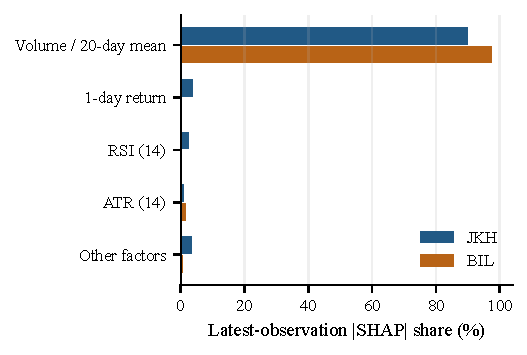
\includegraphics[width=\columnwidth]{shap_shares.pdf}
\caption{Latest-observation absolute SHAP shares for the score surrogate. Remaining supplied features are aggregated as ``Other factors.'' These are not causal price contributions.}
\label{fig:shap}
\end{figure}

JKH had 30 windows and 29 adjacent comparisons, mean ESI 0.896552 and latest ESI 1.0. BIL had 29 windows and 28 comparisons, both mean and latest ESI 1.0. These high readings can partly reflect the score's volume denominator and overlapping windows; they are not independent evidence of explanation fidelity or investor understanding.

\section{Integration, Contributions and Limitations}
An authenticated analysis refreshes available history, invokes a new market run and returns dated evidence: prices, deviations, scores, cutoffs, flags, ranges, attributions and limitations. Temporary market inputs are removed after use; archived forecasts are not substituted for live analysis. The current Component 1 regression suite passed 38 tests on 24 October 2026; software checks do not establish predictive accuracy.

The first author developed the market modelling, anomaly, explanation and validation work. K. C. S. Fernando contributed annual/quarterly report interpretation; Harithra K contributed news and sentiment analysis; T. G. R. N. S. Wijesooriya contributed external-market risk using stock data, gold, oil and VIX. Kapila Dissanayaka and Mahima Weerasinghe supervised the project. Their integration supplies a unified explanation; the present empirical results evaluate only the market contribution.

The principal limitations are retrospective proxy-label leakage, unverified forecast-registration timing, two stocks and one three-month scenario, and only nine/two test positives. Later rolling-label and horizon upgrades do not retrospectively validate these archived metrics. Corporate actions and volume definitions are not systematically reconciled across the secondary-source histories. Neural weight checkpoints and repeated-seed experiments were not retained. SHAP additivity is not surrogate fidelity; formal interactions and sign-sensitive stability were not established. No controlled comprehension study or trading-profitability evaluation was completed.

\noindent\parbox{\columnwidth}{A non-anomalous day can still occur within a sustained decline. Neither its pattern gap nor an external-news association establishes a price the stock would reach if a conflict ended. Future work requires independent event adjudication, nested temporal tests, timestamp-locked forecasts, interval scoring and measured human understanding. Outputs support investigation, not buying or selling advice.}\par

\newpage
\section{Conclusion}
The workflow connects expected prices, volume-adjusted deviations, calibrated alerts and traceable surrogate explanations. Preserved experiments show baseline forecast superiority, a recall--false-alarm trade-off and stable but volume-dominated explanations. The contribution is an auditable CSE evidence pipeline, not demonstrated predictive superiority. Independent labels, additional forecast origins and investor-comprehension testing are needed before broader claims.

Future evaluation should freeze data, code, fitted parameters and thresholds before issuing forecasts, then score repeated origins against persistence. Independently reviewed events should support validation-retuned comparisons of the liquidity rule, band rule and their combination. This would establish whether participation adjustment adds useful detections rather than additional alerts. Explanation assessment should check surrogate fidelity and users' ability to distinguish association, uncertainty and causation.

\begin{thebibliography}{00}
\bibitem{hochreiter} S. Hochreiter and J. Schmidhuber, ``Long short-term memory,'' \textit{Neural Computation}, vol. 9, no. 8, pp. 1735--1780, 1997, doi: 10.1162/neco.1997.9.8.1735.
\bibitem{fischer} T. Fischer and C. Krauss, ``Deep learning with long short-term memory networks for financial market predictions,'' \textit{European Journal of Operational Research}, vol. 270, no. 2, pp. 654--669, 2018, doi: 10.1016/j.ejor.2017.11.054.
\bibitem{hyndmanbook} R. J. Hyndman and G. Athanasopoulos, \textit{Forecasting: Principles and Practice}, 3rd ed. Melbourne, Australia: OTexts, 2021. [Online]. Available: \url{https://otexts.com/fpp3/}
\bibitem{hyndmankoehler} R. J. Hyndman and A. B. Koehler, ``Another look at measures of forecast accuracy,'' \textit{International Journal of Forecasting}, vol. 22, no. 4, pp. 679--688, 2006, doi: 10.1016/j.ijforecast.2006.03.001.
\bibitem{chandola} V. Chandola, A. Banerjee, and V. Kumar, ``Anomaly detection: A survey,'' \textit{ACM Computing Surveys}, vol. 41, no. 3, Art. no. 15, 2009, doi: 10.1145/1541880.1541882.
\bibitem{isolation} F. T. Liu, K. M. Ting, and Z.-H. Zhou, ``Isolation forest,'' in \textit{Proc. IEEE International Conference on Data Mining}, 2008, pp. 413--422, doi: 10.1109/ICDM.2008.17.
\bibitem{amihud} Y. Amihud, ``Illiquidity and stock returns: Cross-section and time-series effects,'' \textit{Journal of Financial Markets}, vol. 5, no. 1, pp. 31--56, 2002, doi: 10.1016/S1386-4181(01)00024-6.
\bibitem{saito} T. Saito and M. Rehmsmeier, ``The precision-recall plot is more informative than the ROC plot when evaluating binary classifiers on imbalanced datasets,'' \textit{PLOS ONE}, vol. 10, no. 3, Art. no. e0118432, 2015, doi: 10.1371/journal.pone.0118432.
\bibitem{shap} S. M. Lundberg and S.-I. Lee, ``A unified approach to interpreting model predictions,'' in \textit{Advances in Neural Information Processing Systems}, vol. 30, 2017, pp. 4765--4774.
\bibitem{treeshap} S. M. Lundberg \textit{et al.}, ``From local explanations to global understanding with explainable AI for trees,'' \textit{Nature Machine Intelligence}, vol. 2, pp. 56--67, 2020, doi: 10.1038/s42256-019-0138-9.
\bibitem{breiman} L. Breiman, ``Random forests,'' \textit{Machine Learning}, vol. 45, pp. 5--32, 2001, doi: 10.1023/A:1010933404324.
\bibitem{miller} T. Miller, ``Explanation in artificial intelligence: Insights from the social sciences,'' \textit{Artificial Intelligence}, vol. 267, pp. 1--38, 2019, doi: 10.1016/j.artint.2018.07.007.
\bibitem{adam} D. P. Kingma and J. Ba, ``Adam: A method for stochastic optimization,'' in \textit{Proc. International Conference on Learning Representations}, 2015. [Online]. Available: \url{https://arxiv.org/abs/1412.6980}
\end{thebibliography}
\end{document}
